\chapter{\textit{User Personas}}
\label{apx:personas}

A continuación se reproducen los tres perfiles de usuario (\textit{personas}) completos, construidos a partir de los hallazgos del \textit{User Research} (Capítulo~\ref{ch:user_research}): \textbf{Santiago} (Estudiante) y \textbf{Laura} (Docente/Evaluadora), que corresponden a los dos actores funcionales definidos en el análisis de requerimientos (Capítulo~\ref{ch:requerimientos}), y \textbf{Marcela} (Coordinadora de educación a distancia), que representa a la institución que adopta y gestiona la herramienta. Las frases síntesis y los atributos de cada perfil fueron construidos a partir de los hallazgos del estudio y no corresponden a citas textuales de un participante individual; las fotografías son imágenes de banco utilizadas únicamente a fines ilustrativos del perfil, sin correspondencia con ninguna persona real relevada durante la investigación. El material editable de estos perfiles se encuentra disponible en Canva: \url{https://canva.link/i8bsiyo7faatefb}.

\begin{figure}[p]
    \centering
    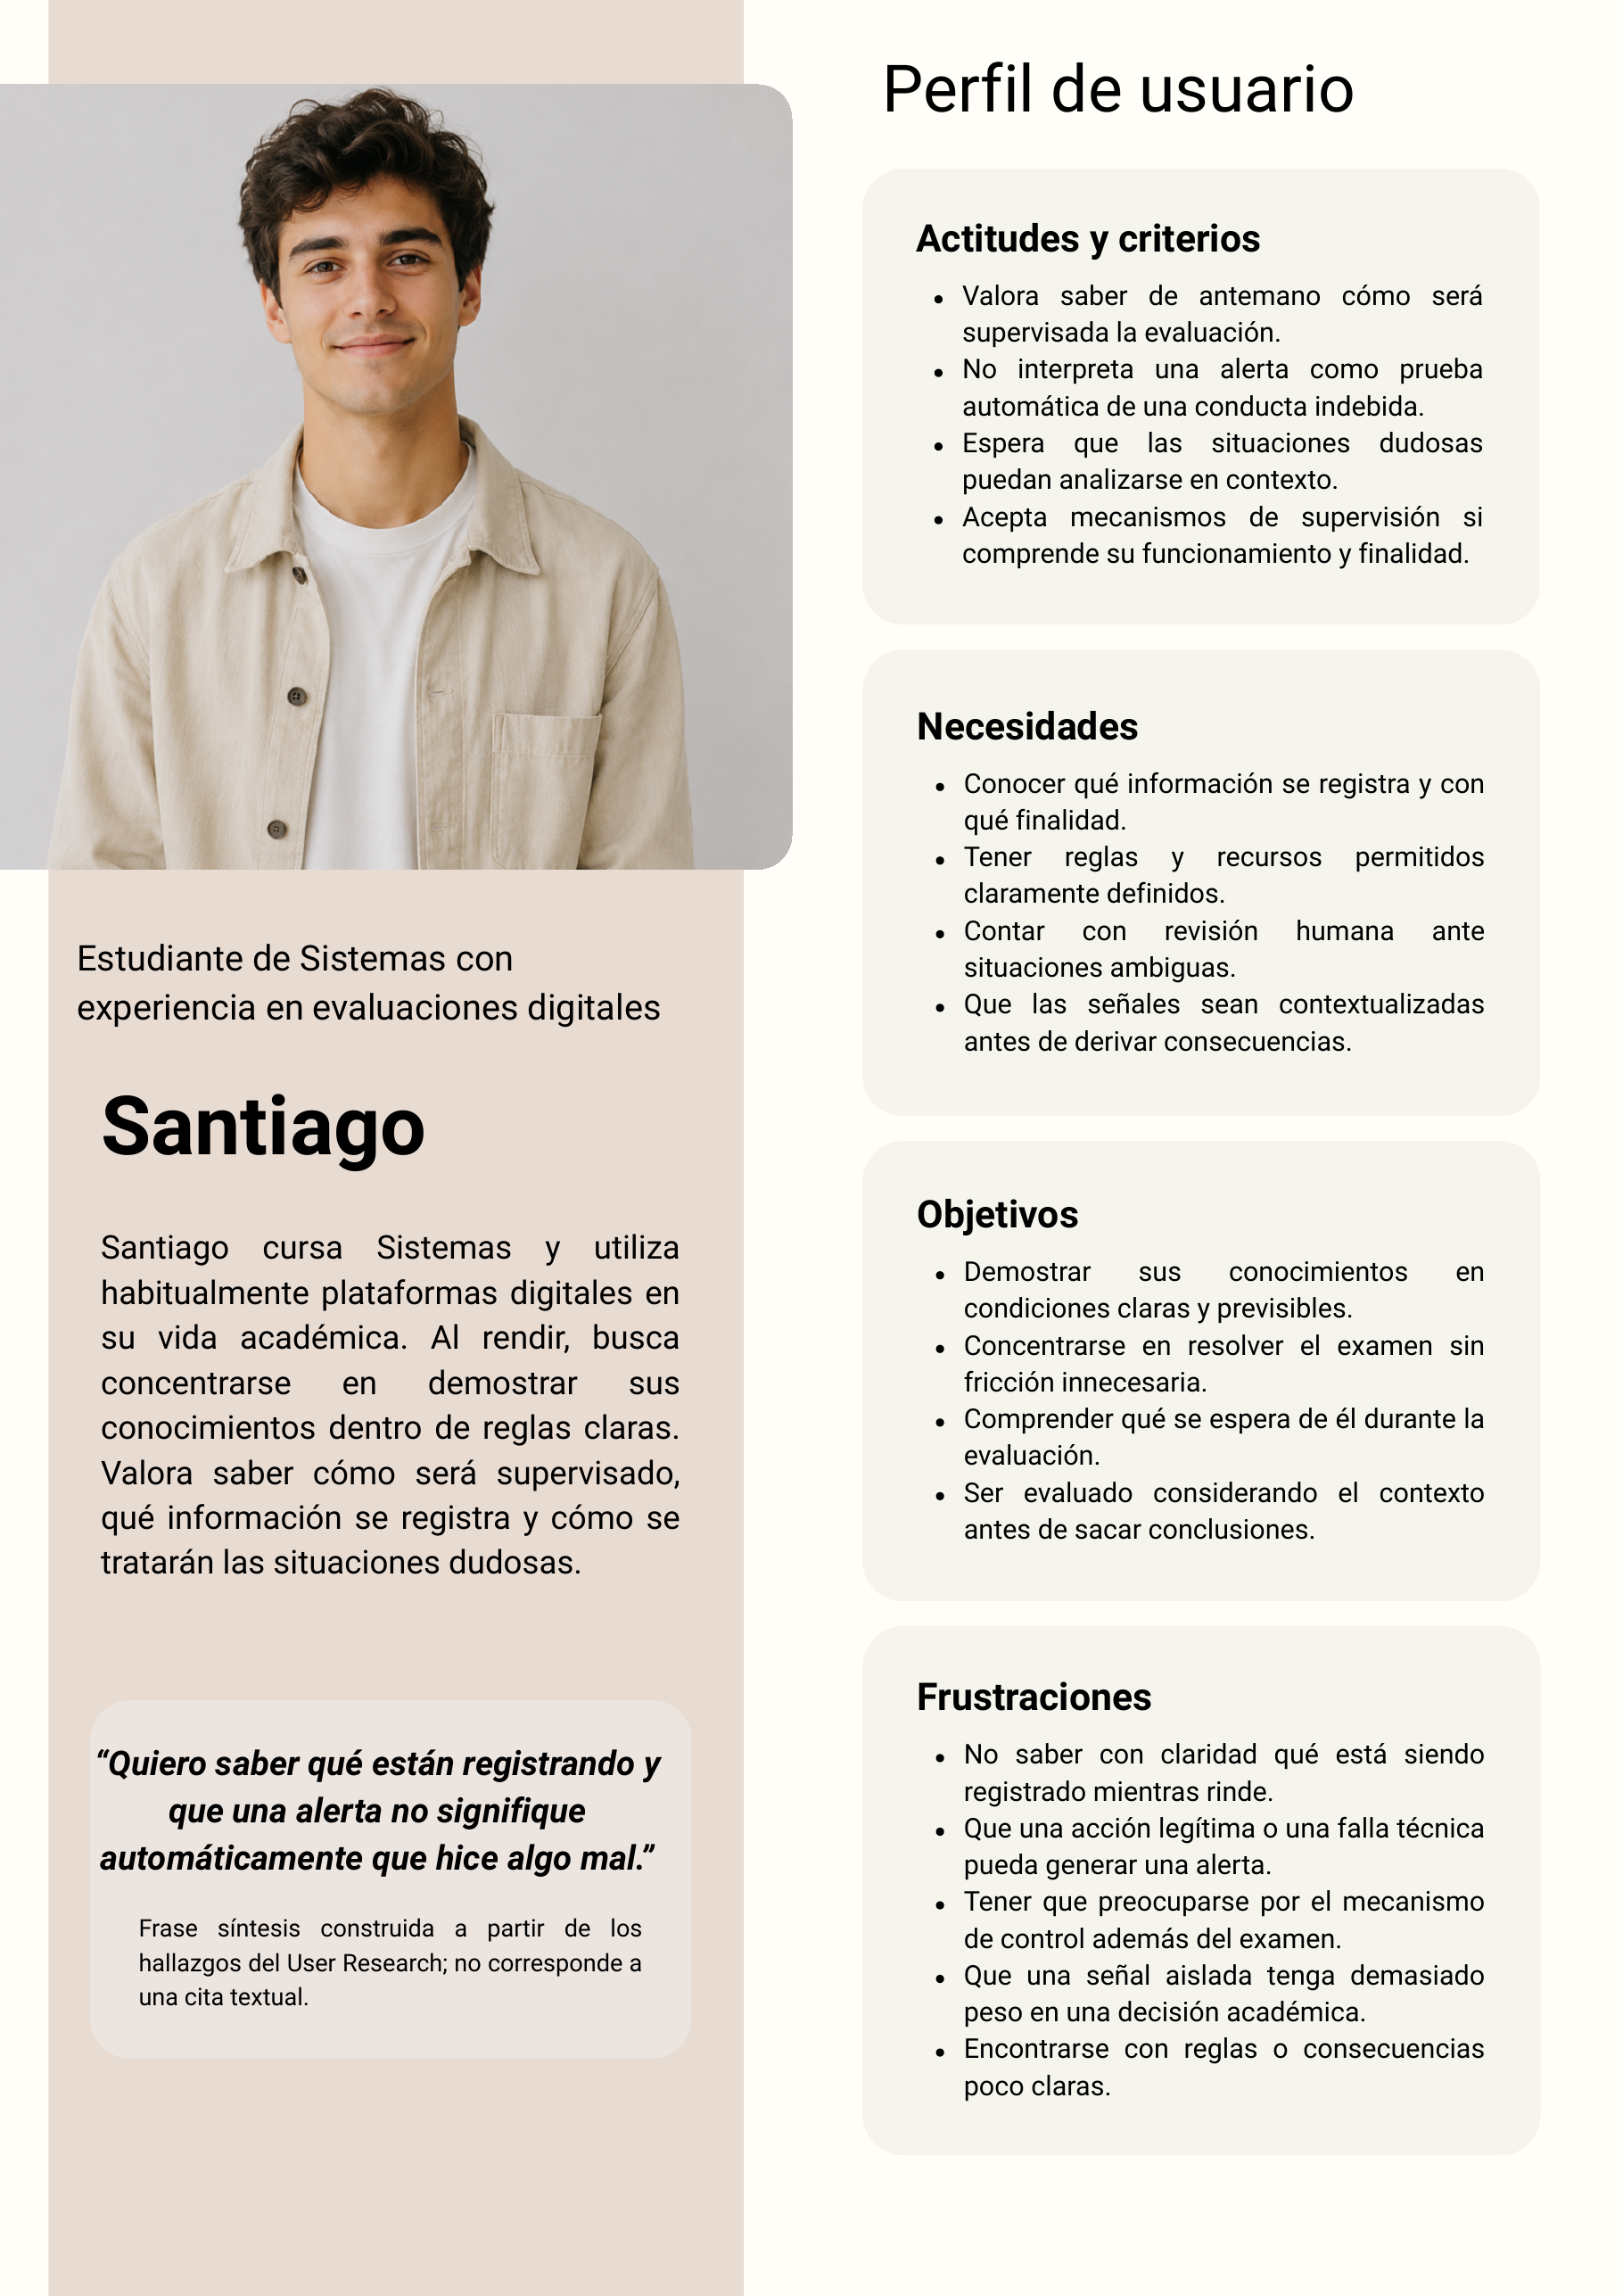
\includegraphics[width=0.95\textwidth]{./figures/persona_santiago.png}
    \caption[Perfil de usuario --- Santiago, Estudiante de Sistemas con experiencia en evaluaciones digitales]{Perfil de usuario --- Santiago, Estudiante de Sistemas con experiencia en evaluaciones digitales. Fuente: elaboración propia a partir del \textit{User Research}.}
\end{figure}

\begin{figure}[p]
    \centering
    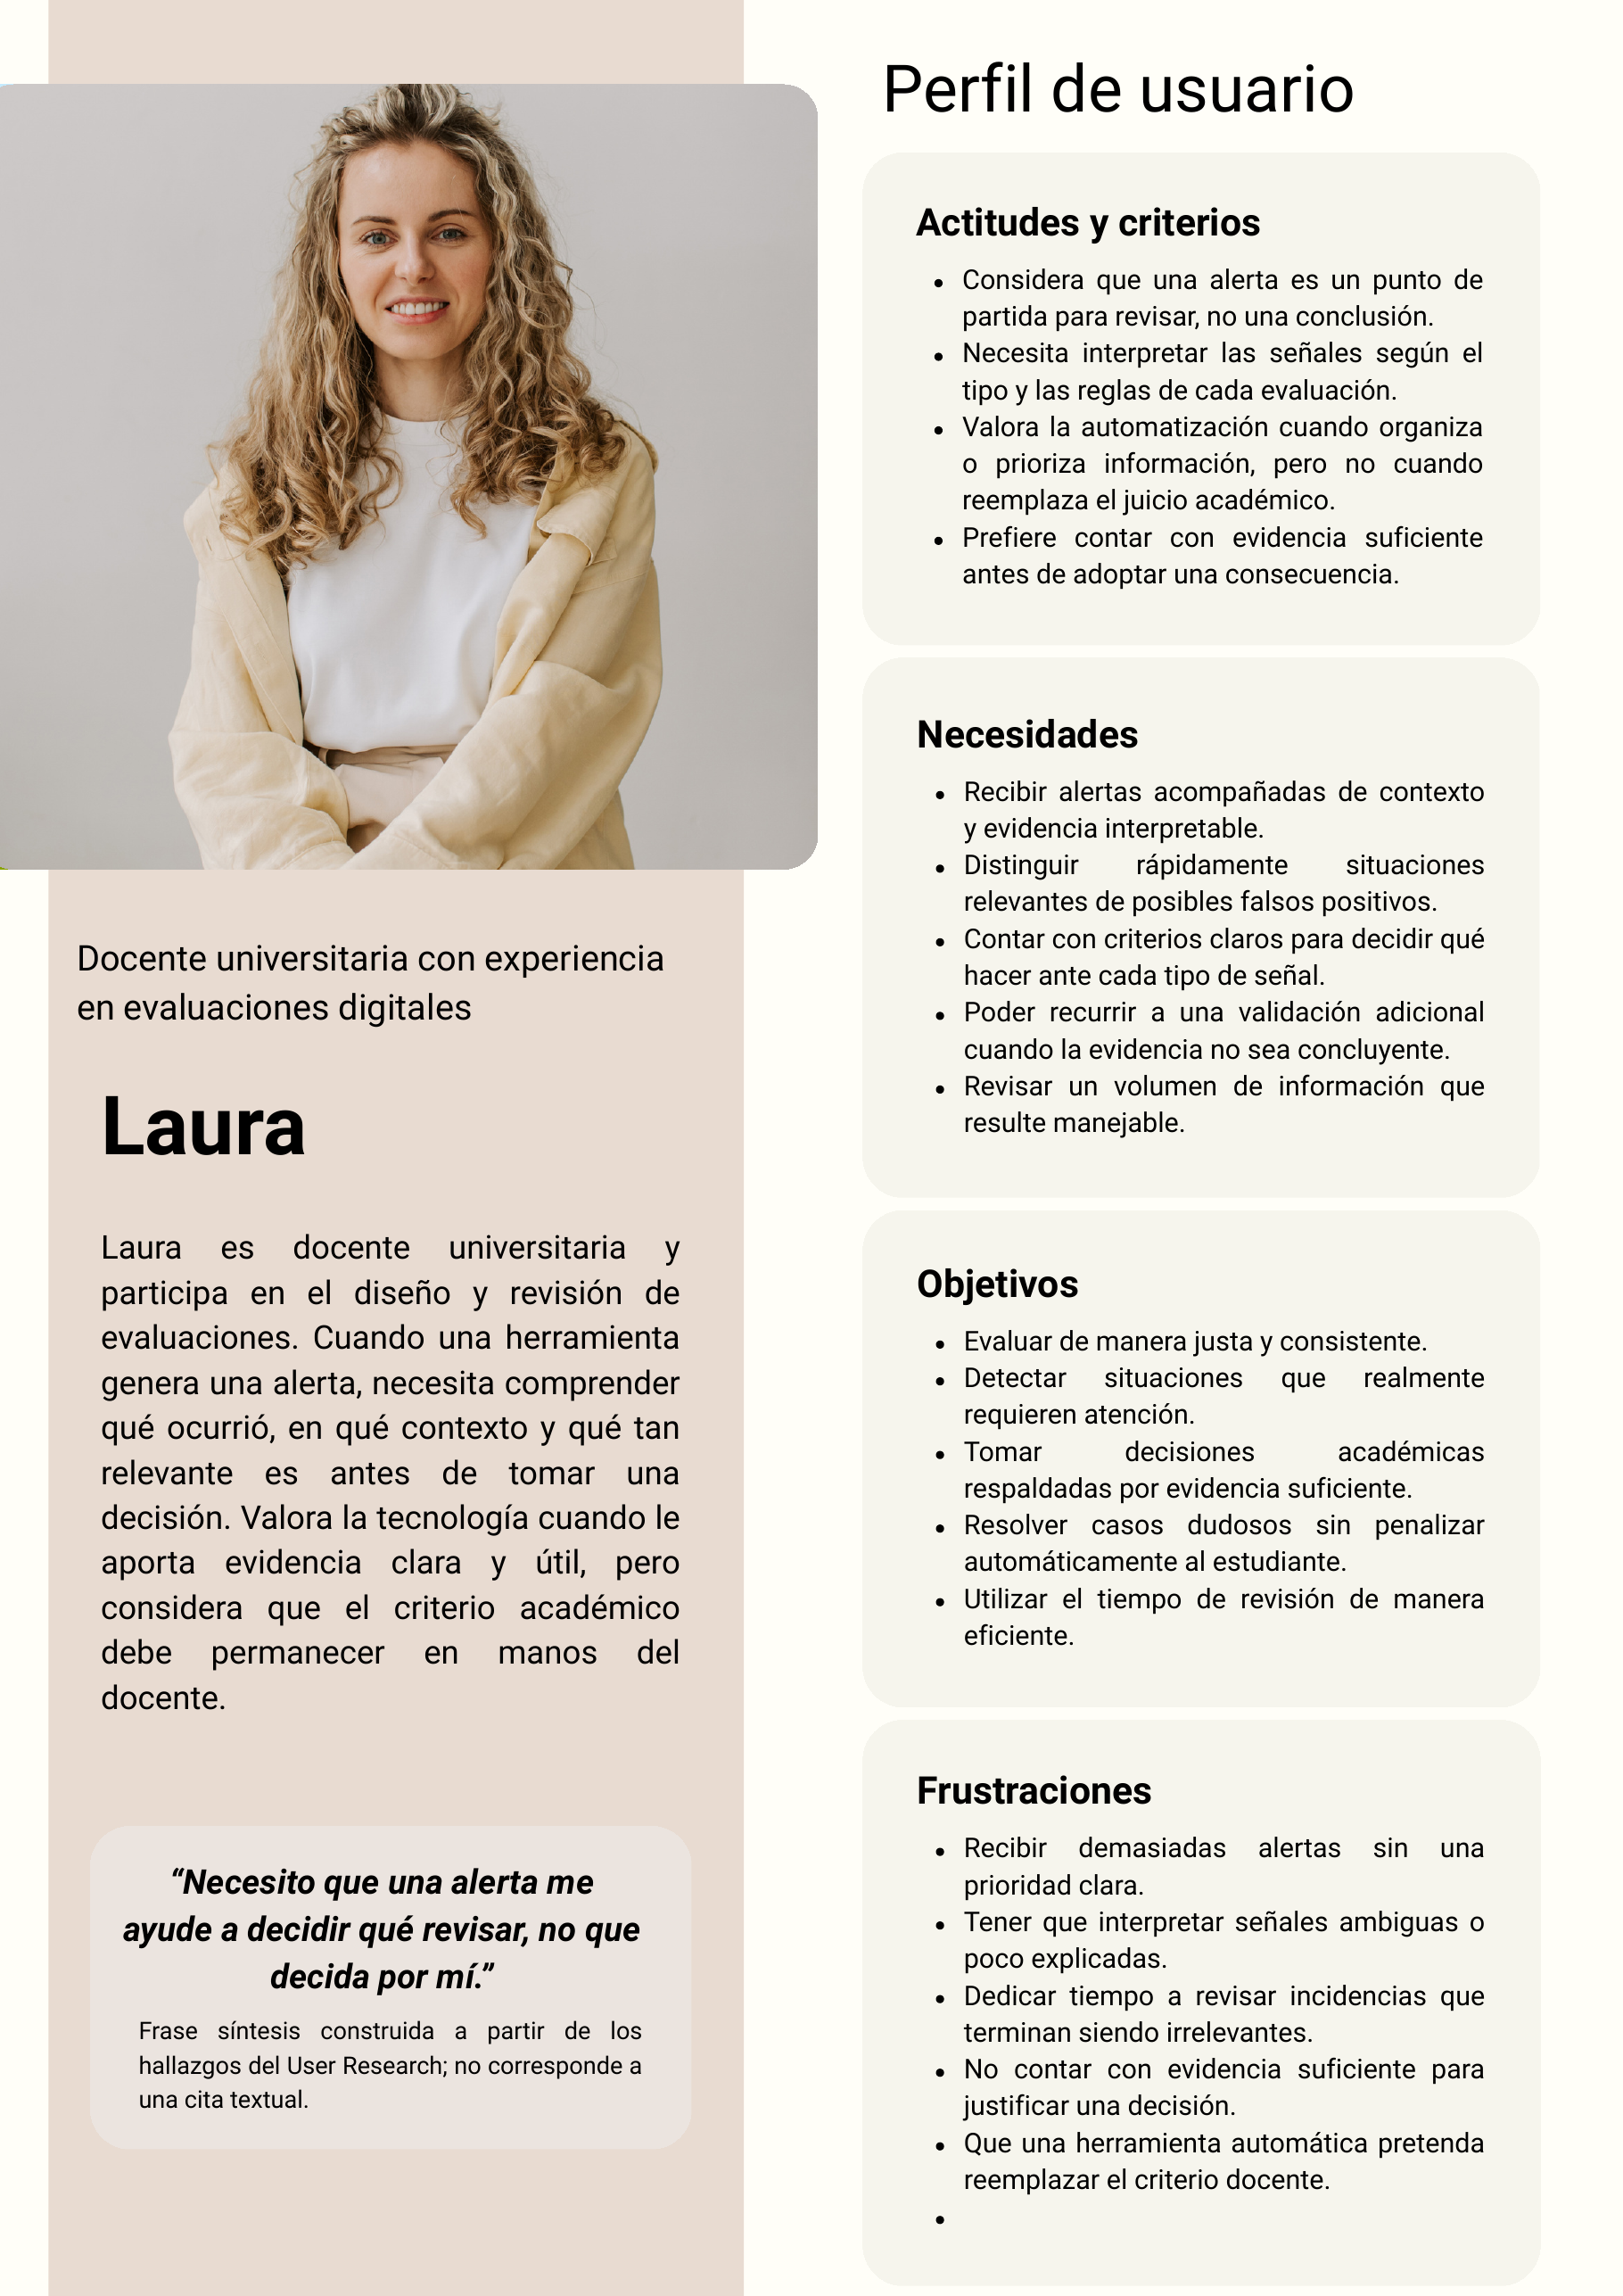
\includegraphics[width=0.95\textwidth]{./figures/persona_laura.png}
    \caption[Perfil de usuario --- Laura, Docente universitaria con experiencia en evaluaciones digitales]{Perfil de usuario --- Laura, Docente universitaria con experiencia en evaluaciones digitales. Fuente: elaboración propia a partir del \textit{User Research}.}
\end{figure}

\begin{table}[p]
    \caption{Perfil de usuario --- Marcela, Coordinadora de educación a distancia}
    \label{tab:persona_marcela}
    \centering
    \small
    \begin{tabularx}{\textwidth}{p{3.2cm} X}
        \toprule
        \tblhead \textbf{Atributo} & \textbf{Descripción} \\
        \midrule
        Perfil & 45 años. Coordina el área de educación a distancia de una universidad privada: define lineamientos de evaluación en línea, gestiona las herramientas de la plataforma y capacita a los docentes. \\
        Frase síntesis & ``Lo que se registra en un examen tiene que poder explicarse y sostenerse ante un reclamo, y no puede sumarles a los docentes más trabajo del que pueden gestionar.'' \\
        Actitudes y criterios & Considera que la curaduría humana de cualquier resultado automatizado es indispensable; desconfía de las incidencias que surgen de contingencias técnicas del entorno del estudiante; evalúa cada herramienta por la relación entre la información que aporta y los recursos que demanda. \\
        Necesidades & Lineamientos claros sobre qué se registra y para qué; información que los docentes puedan interpretar con una capacitación razonable; criterios que permitan justificar una acción académica. \\
        Objetivos & Sostener la confianza en las evaluaciones digitales de la institución; reducir los reclamos por incidencias sin fundamento; escalar las evaluaciones en línea sin aumentar proporcionalmente la carga docente. \\
        Frustraciones & Falsos positivos por notificaciones, cortes de conexión o movimientos del entorno; docentes sin autonomía para interpretar reportes; volúmenes de alertas que no pueden revisarse. \\
        Fuentes & Entrevistas a ENT-01 y a ENT-03 (Apéndice~\ref{apx:entrevistas}); códigos FP-CONT, REV-HUM, EVID-ACT y CARGA-ESC del análisis cualitativo (Apéndice~\ref{apx:cualitativo}). Sin respaldo de encuesta. \\
        \bottomrule
    \end{tabularx}
\end{table}
